\documentclass[12pt, a4paper, twoside]{article}

%% Preamble
\usepackage{umatfgspanish}
\usepackage{tabto}
\newcommand\ttab{\tab \hspace{-5cm}}

\graphicspath{{./images/}}

\begin{document}

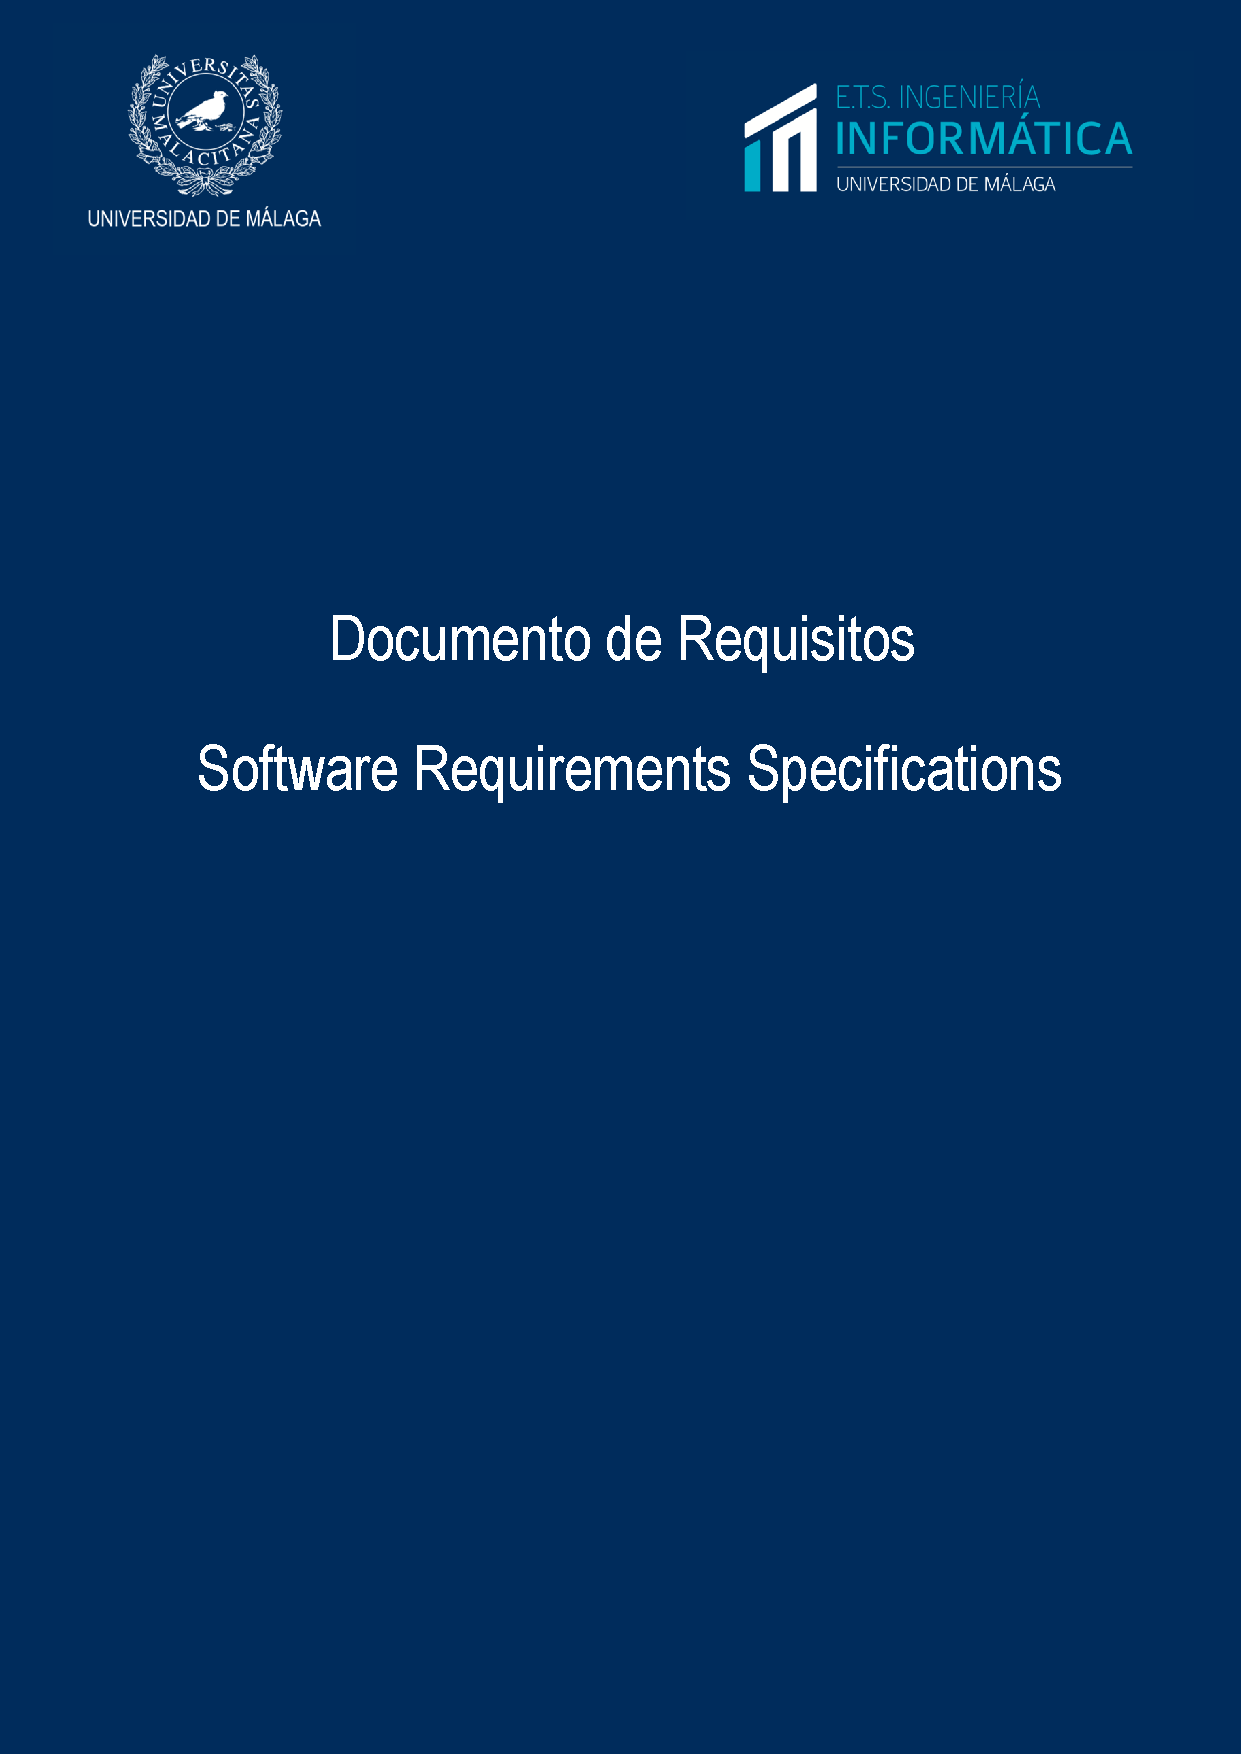
\includepdf[noautoscale=true, width=\paperwidth]{title.pdf}

\newpage

\tableofcontents

%% Sections
\section{Síntesis del documento}
\section{Propósito}
\subsection{Propósito}
Desarrollar un Software que permita interactuar con cualquier elemento 
integrable a la red de Internet que se encuentre en un edificio.
\section{Proceso de Análisis del Negocio}
\section{Ámbito}
Debido a las características del software que hacen uso de las tecnologías 
\"Internet de las Cosas\" (IoT) para la gestión de dispositivos conectados a
la red de un Edificio Inteligente (Smart Building), se ha decidido darle el nombre de
\"IoTBuildingManagement\".

IoTBuildingManagement será el módulo principal al que se podrán conectar diversos pluggins para la
gestión de dispositivos IoT concretos dentro de un edificio. Cada pluggin deberá de tener 
la lógica para controlar los datos de un dispositivo específico.

IoTBuildingManagement deberá tener la lógica necesaria para que los dispositivos IoT
puedan coordinarse entre sí.

\subsection{Preparación para el Análisis del Negocio}
\subsubsection{Contextualización}
El contexto que se va a desarrollar a continuación parte del concepto de Internet de las Cosas (IoT).

Internet consiste en una red de usuarios y servidores conectadas entre sí.
Sin embargo, existen conceptos más amplios que abarcan un conjunto de elementos todavía más ambicioso,
como es el de IoT, que, además de los anteriores, incluye a cualquier objeto físico como participante de la red.

De esta forma podemos ser capaces de interactuar con los objetos de manera remota, sin intervención física de
una persona, o de manera automática.

Además, podrían realizar sus tareas de forma más inteligente, ya que, al estar conectadas a internet, pueden
disponer de mucha información útil para su objetivo.

Desde que se empezó a aplicar el concepto de IoT, se puede ver que ha ocurrido una evolución y ha mejorando en
muchos los aspectos: El presupuesto invertido en la IoT ha incrementado, el número de dispositivos ha crecido
exponencialmente, ...

También es destacable mencionar que la situación global de la COVID-19 ha incentivado y acelerado la aplicación
de la IoT en diversos aspectos como la salud pública, la seguridad o la privacidad.
(
En los últimos años, el uso del IoT ha aumentado exponencialmente [ENSEÑAME LO QUE TIENES].
Elnashar, A. \& El-saidny, M. (2018). IoT evolution towards a super-connected world. Wiley. \textit{Practical Guide to LTE-A, VoLTE and IoT: Paving the way towards 5G}. pp. 310-381. Wiley. https://doi.org/10.1002/9781119063407.ch7
Ayman Elnashar; Mohamed A. El-saidny, "IoT Evolution Towards a Super‐connected World," in Practical Guide to LTE-A, VoLTE and IoT: Paving the way towards 5G , Wiley, 2018, pp.310-381, doi: 10.1002/9781119063407.ch7.

)
\subsubsection{Problemas y oportunidades identificadas}
REF: 
Estevez E., Pardo, T., \& Scholl, J. (2021). Smart cities and smart governance: towards the 22nd century sustainable city. Springer.

La IoT es una tecnología relativamente reciente y son muchos los campos los que se pueden beneficiar de su uso:
ciudades inteligentes, agricultura, Smart Home, 
Una oportunidad identificada es el hecho de que el IoT es una tecnología muy reciente y todavía
no se ha aplicado en numerosos campos 
\section{Introducción}
\subsection{Definiciones}
\begin{itemize}
    \item \textbf{Sensores}\ttab Los sensores son dispositivos IoT cuya labor principal es recolectar datos.
    \item \textbf{Actuadores}\ttab Los actuadores son dispositivos IoT cuya función principal hacer una tarea.
  \end{itemize}
\subsection{Acrónimos y Abreviaturas}
\begin{itemize}
    \item \textbf{IoT}\ttab Internet de las Cosas
  \end{itemize}

\section{Análisis del proyecto}
\subsection{Contextualización}
El trabajo que se va a desarrollar a continuación toma como concepto base el Internet de las Cosas (IoT).
Esta idea consiste en tener en cuenta, como usuarios de internet, a un conjunto más amplio que el 
habitual. Es decir, no solo incluye a personas y a servidores tradicionales, sino también trata a cualquier objeto 
físico como un candidato válido a formar parte del sistema.

Entre de las ventajas más destacadas a la hora de usar IoT, podemos mencionar:
\begin{itemize}
    \item La sensorización: Permite obtener datos que anteriormente no podían ser recogidos de manera automática.
    \item Acciones remotas: Los objetos que se conectan a la red pueden realizar acciones físicas desencadenadas por internet,
      por lo que no tiene haber nadie presente ante el objeto para poder manipularlo o monitorizar su estado.
    \item Interacción entre dispositivos IoT: Gracias a los modelos de comunicación, se pueden realizar tareas complejas
      comunicando diferentes sensores y actuadores, de esta forma, se producen una secuencia de acciones sin necesidad
      de intervención humana, que produce unos resultados dignos de categorizar como inteligentes.
\end{itemize}

\subsubsection{Problemática y oportunidades identificadas}
De acuerdo con (Estevez et al., 2021), la densidad de población que habita en las ciudades crece aceleradamente.
Se espera que para el 2030, un 60\% de las personas viva en las ciudades. 

Al existir una migración tan importante de áreas rurales a urbanas, el entorno de la
propia ciudad evoluciona más rápido y los retos a los que estas se enfrentan, o se espera que se enfrenten,
también cambian notablemente: el transporte, impacto medioambiental, salud pública, servicios, etc. Son puntos
críticos que merecen especial atención para mantener y mejorar el funcionamiento y la calidad de vida en
las urbes.

Todo esto sumado al crecimiento de las infraestructuras de telecomuncación (Banda ancha, wifi y 5G)
y a las inversiones en inteligencia artificial y big data, abre la posiblidad de aplicar el IoT como
posible solución y ofrecer mejoras a los gobiernos y ciudadanos, que ayuden a mejorar la gestión de las 
ciudades, mejoren la calidad de vida en las mismas y sean lo más respetuosas con el entorno.

Estevez E., Pardo, T., \& Scholl, J. (2021).
Smart cities and smart governance: towards the 22nd century sustainable city. Springer.


Otra motivación para usar el IoT viene de que se trata de  una tecnología relativamente reciente 
y son muchos los campos en los que se puede aplicar para sacar ventaja.

El potencial que se le puede sacar a esta red de dispositivos es muy elevado. Existen conceptos tales como:
 - IoT Orchestation
 - Fog Computing

que pueden aportar a una transformación digital inteligente y sostenible de las ciudades.


 ---------------------

Por otro lado, cuando se analiza cuál ha sido el avance del IoT desde sus comienzos,
se puede llegar a la conclusión de que ha avanzado muy rápido, y todavía hay muchos 
puntos en los que debe de madurar:
 - Interfaces de Estandarización (Discovery, semántica de datos)
 - Data Swamp (Discovery)

Por lo que a la hora de hacer un desarrollo usando IoT se deben de tener en cuenta estos aspectos.

\section{Propósito}
Uno de los objetivos de este sistema será el de ofrecer una plataforma común que
permita interconectar dispositivos de la Smart City usando interfaces que ya son estándar.

Según el punto de vista de Fiware, las ciudades tienen 5 etapas en su camino a la digitalización inteligente:
 -
 -
 -
 -
 -



 \section{Ámbito}
 Describe the scope of the software under consideration by:
 a) identifying the software product(s) to be produced by name (e.g., Host DBMS, Report Generator, etc.);
 b) explaining what the software product(s) will do;
 c) describing the application of the software being specified, including relevant benefits, objectives
 and goals; and
 d) being consistent with similar statements in higher-level specifications (e.g., a system requirements
 specification), if they exist.

 \section{Perspectiva del Producto}
 Define the system's relationship to other related products.
 If the product is an element of a larger system, relate the requirements of that larger system to the
 functionality of the product covered by the SRS.
 If the product is an element of a larger system, identify the interfaces between the product covered by
 the SRS and the larger system of which the product is an element.
 Consider a block diagram showing the major elements of the larger system, interconnections and
 external interfaces.
 Describe how the software operates within the following constraints:
 a) system interfaces;
 b) user interfaces;
 c) hardware interfaces;
 d) software interfaces;
 e) communications interfaces;
 f) memory;
 g) operations;
 h) site adaptation requirements; and
 i) interfaces with services.

 \subsection{Interfaces del Sistema}
 List each system interface and identify the functionality of the software to accomplish the system
 requirement and the interface description to match the system.

 \subsection{Interfaces de Usuario}
 Specify the logical characteristics of each interface between the software product and its users.
 NOTE A style guide for the user interface can provide consistent rules for organization, coding and
 interaction of the user with the system.

 \subsection{Interfaces Hardware}
 Specify the logical characteristics of each interface between the software product and the hardware
 elements of the system. This includes configuration characteristics (number of ports, instruction sets,
 etc.). It also covers such matters as what devices are to be supported, how they are to be supported, and
 protocols. For example, terminal support may specify full-screen support as opposed to line-by-line
 support.

 \subsection{Interfaces Software}
 Specify the use of other required software products (e.g., a data management system, an operating
 system or a mathematical package), and interfaces with other application systems (e.g., the linkage
 between an accounts receivable system and a general ledger system).
 For each required software product, specify:
 a) name;
 b) mnemonic;
 c) specification number;
 d) version number; and
 e) source.
 NOTE It is acceptable to specify required platforms or operating systems, but rarely feasible to require a
 specific version. Typically, a version number most recent version or any currently maintain version can be
 specified for software.
 For each interface, specify:
 a) discussion of the purpose of the interfacing software as related to this software product;
 b) definition of the interface in terms of message content and format. It is not necessary to detail any
 well-documented interface, but a reference to the document defining the interface is required.

 \subsection{Interfaces de Comunicación}
 Specify the various interfaces to communications such as local network protocols.

 \subsection{Restricciones de Memoria}
 Specify any applicable characteristics and limits on primary and secondary memory.

 \subsection{Operaciones}
 Specify the normal and special operations required by the user such as:
 a) the various modes of operations in the user organization (e.g., user-initiated operations);
 b) periods of interactive operations and periods of unattended operations;
 c) data processing support functions; and
 d) backup and recovery operations.
 NOTE This is sometimes specified as part of the User Interfaces section.

 \subsection{Site adaptation requirements}
 The site adaptation requirements include:
 a) definition of the requirements for any data or initialization sequences that are specific to a given
 site, mission or operational mode (e.g., grid values, safety limits, etc.);
 b) specification of the site or mission-related features that should be modified to adapt the software
 to a particular installation.

 \subsection{Interfaces with services}
 Specify interactions with services, e.g., Software as a Service (SaaS) or cloud services.

 \section{Funciones del producto}
 Provide a summary of the major functions that the software will perform. For example, an SRS for an
 accounting program may use this part to address customer account maintenance, customer statement
 and invoice preparation without mentioning the vast amount of detail that each of those functions
 requires.
 Sometimes the function summary that is necessary for this part can be taken directly from the section
 of the higher-level specification (if one exists) that allocates particular functions to the software
 product.
 Use cases, user stories and scenarios are also used to describe product functions.
 Note that for the sake of clarity:
 a) the product functions should be organized in a way that makes the list of functions understandable
 to the acquirer or to anyone else reading the document for the first time.
 b) textual or graphical methods can be used to show the different functions and their relationships.
 Such a diagram is not intended to show a design of a product, but simply shows the logical
 relationships among variables.

 \section{Características de los Usuarios}
 Describe those general characteristics of the intended groups of users of the product including
 characteristics that may influence usability, such as educational level, experience, disabilities and
 technical expertise. This description should not state specific requirements, but rather should state the
 reasons why certain specific requirements are later specified in specific requirements in 9.6.9.
 NOTE 1 Where appropriate, the user characteristics of the SyRS and SRS are consistent.
 NOTE 2 For additional information on context of use and user needs, see ISO/IEC 25063 and ISO/IEC 25064.

 \section{Limitaciones}
 Provide a general description of any other items that will limit the supplier's options, including:
 a) regulatory requirements and policies;
 b) hardware limitations (e.g., signal timing requirements);
 c) interfaces to other applications;
 d) parallel operation;
 e) audit functions;
 f) control functions;
 g) higher-order language requirements;
 h) signal handshake protocols (e.g., XON-XOFF, ACK-NACK);
 i) quality requirements (e.g., reliability);
 j) criticality of the application;
 k) safety and security considerations;
 l) physical/mental considerations; and
 m) limitations that are sourced from other systems, including real-time requirements from the
 controlled system through interfaces.

 \section{Suposiciones y dependencias}
 List each of the factors that affect the requirements stated in the SRS. These factors are not design
 constraints on the software but any changes to these factors can affect the requirements in the SRS.
 For example, an assumption may be that a specific operating system will be available on the hardware
 © ISO/IEC 2018 – All rights reserved
 70 © IEEE 2018 – All rights reserved
 Authorized licensed use limited to: Universidad de Malaga. Downloaded on July 13,2022 at 15:40:49 UTC from IEEE Xplore. Res
 ISO/IEC/IEEE 29148:2018(E)
 designated for the software product. If, in fact, the operating system is not available, the SRS would
 have to change accordingly.

 \section{Apportioning of requirements}
 Apportion the software requirements to software elements. For requirements that will require
 implementation over multiple software elements, or when allocation to a software element is initially
 undefined, this should be so stated. A cross-reference table by function and software element should be
 used to summarize the apportionments.
 Identify requirements that may be delayed until future versions of the system (e.g., blocks and/or
 increments).

 \section{Specified requirements}
 Specify the software system requirements to a level of detail sufficient for software design, development
 and verification of the software increment or release in process.
 The requirements should:
 a) be stated in conformance with all the characteristics described in 5.2 of this document;
 b) be cross-referenced to earlier versions or related documents;
 c) be uniquely identifiable;
 d) describe every input (stimulus) into the software system, every output (response) from the
 software system, and all functions performed by the software system in response to an input or in
 support of an output.

 \section{Interfaces externas}
 Define all inputs into and outputs from the software system. The description should complement the
 interface descriptions in 9.6.4.1 through 9.6.4.5, and should not repeat information there.
 Each interface defined should include the following content:
 a) name of item;
 b) description of purpose;
 c) source of input or destination of output;
 d) valid range, accuracy and/or tolerance;
 e) units of measure;
 f) timing;
 g) relationships to other inputs/outputs;
 h) data formats;
 i) command formats; and
 j) data items or information included in the input and output.

 \section{Funciones}
 Define the fundamental actions that have to take place in the software in accepting and processing the
 inputs and in processing and generating the outputs, including:
 a) validity checks on the inputs;
 b) exact sequence of operations;
 c) responses to abnormal situations, including:
 1) overflow;
 2) communication facilities;
 3) hardware faults and failures; and
 4) error handling and recovery;
 d) effect of parameters;
 e) relationship of outputs to inputs, including:
 1) input/output sequences; and
 2) formulas for input to output conversion.
 It may be appropriate to partition the functional requirements into sub-functions or sub-processes.
 This does not imply that the software design will also be partitioned that way.

 \section{Requisitos de Usabilidad}
 Define usability and quality in use requirements and objectives for the software system that can include
 measurable effectiveness, efficiency, satisfaction criteria and avoidance of harm that could arise from
 use in specific contexts of use.
 NOTE Additional guidance on usability requirements can be found in ISO/IEC TR 25060.

 \section{Requisitos de Rendimiento}
 Specify both the static and the dynamic numerical requirements placed on the software or on human
 interaction with the software as a whole.
 Static numerical requirements may include the following:
 a) the number of terminals to be supported;
 b) the number of simultaneous users to be supported; and
 c) the amount and type of information to be handled.
 Static numerical requirements are sometimes identified under a separate section entitled Capacity.
 Dynamic numerical requirements may include, for example, the numbers of transactions and tasks and
 the amount of data to be processed within certain time periods for both normal and peak workload
 conditions.
 The performance requirements should be stated in measurable terms.
 For example,
 95 \% of the transactions shall be processed in less than 1 s.
 rather than,
 An operator shall not have to wait for the transaction to complete.
 NOTE Numerical limits applied to one specific function are normally specified as part of the processing
 subparagraph description of that function.

 \section{Logical database requirements}
 Specify the logical requirements for any information that is to be placed into a database, including:
 a) types of information used by various functions;
 b) frequency of use;
 c) accessing capabilities;
 d) data entities and their relationships;
 e) integrity constraints;
 f) security; and
 g) data retention requirements.

 \section{Restricciones de Diseño}
 Specify constraints on the system design imposed by external standards, regulatory requirements or
 project limitations.

 \section{Standards compliance}
 Specify the requirements derived from existing standards or regulations, including:
 a) report format;
 b) data naming;
 c) accounting procedures; and
 d) audit tracing.
 For example, this could specify the requirement for software to trace processing activity. Such traces
 are needed for some applications to meet minimum regulatory or financial standards. An audit trace
 requirement may, for example, state that all changes to a payroll database shall be recorded in a trace
 file with before and after values.

 \section{Software system attributes}
 Specify the required attributes of the software product. The following is a partial list of examples:
 a) Reliability - specify the factors required to establish the required reliability of the software system
 at the time of delivery.
 b) Availability - specify the factors required to guarantee a defined availability level for the entire
 system such as checkpoint, recovery and restart.
 c) Security - specify the requirements to protect the software from accidental or malicious access,
 use modification, destruction or disclosure. Specific requirements in this area could include the
 need to:
 1) utilize certain cryptographic techniques;
 2) keep specific log or history data sets;
 3) assign certain functions to different modules;
 4) restrict communications between some areas of the programme;
 5) check data integrity for critical variables; and
 6) assure data privacy.
 d) Maintainability - specify attributes of software that relate to the ease of maintenance of the
 software itself. These may include requirements for certain modularity, interfaces or complexity
 limitation. Requirements should not be placed here just because they are thought to be good design
 practices.
 e) Portability - specify attributes of software that relate to the ease of porting the software to other
 host machines and/or operating systems, including:
 1) percentage of elements with host-dependent code;
 2) percentage of code that is host dependent;
 3) use of a proven portable language;
 4) use of a particular compiler or language subset; and
 5) use of a particular operating system.

 \section{Verificación}
 Provide the verification approaches and methods planned to qualify the software. The information
 items for verification are recommended to be given in a parallel manner with the information items in
 9.6.10 to 9.6.18.
 
 \section{Información de Soporte}
 Additional supporting information to be considered includes:
 a) sample input/output formats, descriptions of cost analysis studies or results of user surveys;
 b) supporting or background information that can help the readers of the SRS;
 c) a description of the problems to be solved by the software; and
 d) special packaging instructions for the code and the media to meet security, export, initial loading
 or other requirements.
 The SRS should explicitly state whether or not these information items are to be considered part of the
 requirements.

\end{document}